
\chapter{Knji"znica in gradniki za Orange}

V okviru diplomske naloge smo razvili tri lo"cene komponente za programerje in
kon"cne uporabnike programa Orange. 

Prva komponenta je programska knji"znica simple\_wbd, ki
omo"goca enostaven dostop do programskega vmesnika indikatorjev in podnebnih
podatkov Svetovne banke. Ta knji"znica je narejena s "cim manj odvisnosti in je 
% TODO ali je python z veliko
namenjena splo"sni uporabi v Python programih. Poudarka pri zasnovi knji"znice 
simple\_wbd sta predvsem enostavnost razsiritve in zanesljivost. Ta cilja
dose"zemo z mehanizmom za vkljucevanje lastne kode v komponente knji"znice
in mehanizmi za popravljanje ali odstranjevanje pokvarjenih podatkov.

Drugi sestavni del je raz"siritev knji"znice simple\_wbd s funkcionalnostmi, 
potrebnimi za la"zje delo v programu Orange. To predvsem zavzema pretvorbo
pridobljenih podatkov v Orange in numpy tabele. Ta sklop je namenjen skriptnemu
delu s programom Orange in je dostopen kot api\_wrapper Python modul. 

Tretji sestavni del je grafi"cni vmesnik za uporabo api\_wrapper modula. Namen
grafi"cnega vmesnika je omogo"citi ne-programerjem dostop do podatkov 
programskega vmesnika Svetovne banke znotraj programa Orange za namen obdelave,
analize in iskanja zakonitosti med podatki.

\section{Knji"znica simple\_wbd}

Knji"znica simple\_wbd programerjem olaj"sa dostop do podatkov programskega 
vmesnika Svetovne banke. Glavna lastnost te knji"znice je zdru"zevanje ve"cjega 
"stevila zahtev po podatkih in enostavna predstavitev dobljenih podatkov. 
Druga lastnost je pretvorba podatkov iz ve"c dimenzij v dvo-dimenzionalno polje,
primerno za uporabo v programu Orange. Glavna vmesnika te knji"znice sta 
IndicatorAPI in ClimateAPI. Prvi omo"goca pridobivanje podatkov iz programskega 
vmesnika indikatorjev Svetovne banke, drugi pa s programskega vmesnika
podnebnih meritev.


%% % moznost razsiritve z dedovanjem dataset razreda.
%% % 
%% 
%% - omo"goca pridobivanje vrednosti za filtre:
%%     - indicator api: drzave in agregati, indikatorji
%%     - climate api: drzave, tipi podatkov, meritveno obdobje 
%% 
%% - Zahteva za podatke vraca dataset objekt ki ponuja surove podatke, ali pa eno
%%   drugo obliko. 2D array ali pa dict.
%% 
%% - Dataset razred lahko tudi poljubno razsirimo.



\subsection{Pomocnik IndicatorAPI}

IndicatorAPI je razred namenjen pridobivanju podatkov indikatorjev razvoja.
Ker ima programski vmesnik Svetovne banke omejitev koliko podatkov lahko
prenesemo z eno poizvedbo, nam ta razred zdru"zuje rezultate vseh poizvedb, ki
so potrebne za prenos celotne zahteve. To poskrbi tako da se po prvi poizvedbi
sprehodi "cez "stevilo preostalih strani (Primer \ref{basic_response}) ki so na voljo. 
Za razliko od obstoje"cih knji"znic\fnurl{https://pypi.python.org/pypi/wbdata}
\fnurl{https://pypi.python.org/pypi/wbpy/2.0.1} za delo s programskim vmesnikom
Svetovne banke, katerih cilj je "cim bolj natan"cno predstaviti programski 
vmesnik, je cilj nase knji"znice le poenostaviti poizvedbe. V ta namen smo s to
knji"znico razsirili programski vmesnik da lahko z enim klicem funkcije 
prenesemo podatke tudi vec kot le enega indikatorja.

Poleg tega da skrbi za prenos vseh strani podatkov, tudi bele"zi "stevilo 
narejenih in "stevilo potrebnih poizvedb za celoten prenos. Do teh "stevil lahko
dostopamo z drugih niti in jih uporabimo za prikaz napredka in preostalega
casa do prenosa celotne zahteve.

Glavne metode ki jih ponuja IndicatorAPI razred so:

\begin{description}  
\item [get\_indicators] vrne seznam vseh mo"znih indikatorjev z imeni, opisi in
      identifikatorji,
\item [get\_countries] vrne seznam drzav in regij s kodami in metapodatki,
\item [get\_dataset] vrne razred (IndicatorDataset) ki vsebuje vse podatke z 
      poizvedbe in metode za oblikovanje predstavitve podatkov: api\_responses,
      as\_list, as\_dict.
\end{description}



Implementirali lastni caching:
 - obstojece knjiznice (vcrpy, requests-cache) za hranjenje narejenih poizdedb so se izkazale za zelo
 pocasne v primeru ko delamo z vecjim stevilom podatkov.
 - nasa resitev se zanasa na edinstvost URL naslovov - za vsak url si shranimo odgovor in ce je
 mlajsi od enega tedna, isti odgovor uporabim pri vsaki poizvedbi za doloceni URL.


mehanizmem za odpravo napak:
 - pridobiti podatke o drzavi za posamezni indikator: 
   - ob manjkajocih id-jih poskusamo dolociti id iz imena
   - ob manjkajocih imenih poskusamo dobiti ime iz id-ja
   - ce ni nobene informacije ta podatek ignoriramo.

ko zelimo dobiti polje v obliki casovne vrste:
 - pridobivanje datuma iz polja 'date'
   - ob neveljavnih stringih probamo upostevati le zacetni del.
     - za text za  obdobje  '2002 - 2006' bomo uporabili le datum 2002 
   - neveljavne stringe kot so "most rescent value" ignoriramo.







\subsubsection{Razred IndicatorDataset}

Razred IndikatorDataset je osnovni razred v katerem dobimo zahtevane podatke
indikatorjev. Ta razred vsebuje vse potrebne metode in podatke za predstavitev
rezultatov programskega vmesnika, na dva glavna nacina; kot slovar slovarjev in
dvo dimenzionalen seznam. Poleg omenjenih nacinov predstavitve podatkov lahko
dostopamo tudi do neobdelanih podatkov prejetih z programskega vmesnika za
vsako poizvedbo posebej.


Posamezne vrednosti teh podatkov so dolo"cene z drzavo, casovno komponento, in
kodo indikatorja. Te podatke lahko predstavimo na dva glavna nacina:

 - kot gnezdeni slovar, kjer je na prvem nivoju ime indikatorja, na drugem
   drzava, in na tretjem nivoju casovna komponenta.

 - Kot dvo-dimenzionalno polje, kjer imamo v vrsticah eno oznako, v stolpcih
   pa kartezicni produkt ostalih dveh. ponujene moznosti so:
   - vrstice = drzava, stolpci = cas x indikator
   - vrstice = cas, stolpci = drzava x indikator


Indicator



% notes:
% 3 dimenzije: cas, drzava, indikator > vrednost
% 
% lahko damo v:
% 
% 
%    \    drzava x indikator
%   cas
% 
%  ali: 
% 
%    \    cas x indikator
% drzava
% 




\subsection{Pomcnik ClimateAPI}

IndicatorAPI je 


api dovoli le podatke za en tip za eno vrsto obdobja in eno drzavo hkrati.
mi naredim kartezicni produkt med vsemi temi zgradimo vse url-je in naredimo
vse potrebne poizvedbe za pridobitev podatkov.



\subsubsection{Razred IndicatorDataset}

Isto kot pri indicator apiju
ko zelimo dobiti polje v obliki casovne vrste:
 - pridobivanje datuma iz polja 'date'
   - ob neveljavnih stringih probamo upostevati le zacetni del.
     - za text za  obdobje  '2002 - 2006' bomo uporabili le datum 2002 
   - neveljavne stringe kot so "most rescent value" ignoriramo.




as\_dict 

glede na poizvedbo dobimo tu gnezden slovar s polji

drzava / tip podatkov / tip casovnega obdobja / vrednost casovnega obdobja / vrednost

as\_list

% notes:
% 3 dimenzije: cas (decade,year,month), drzava, tip (pr/ tas)
% 
% lahko damo v poljubno konfiguracijo z nastetimi elementi v stolpcu
% 
% stolpci = [drzava, cas] => vrstice = tip ... naredi kartezicni produkt



\section{api\_wrapper}

% doda as orange table in as numpy obema indikator apiju in climate apiju.


raz"siritev simple wbd vmesnikov z dedovanjem pravega dataset razreda.

\begin{verbatim}

class ClimateDataset(simple_wbd.ClimateDataset):
    
    def as_numpy(self):
        raise NotImplemented()
    
    def as_orange_table(self):
        raise NotImplemented()

class ClimateAPI(simple_wbd.ClimateAPI):

    def __init__(self):
        super().__init__(ClimateDataset)
\end{verbatim}


- razsiri as\_list v as\_numpy\_array ki tudi odstrani vse stolpce ki nimajo 
  veljavne vrednosti.

- doda as orange table ki numpy array spremeni v orange tabelo.
  - za indikator api doda se metapodatke drzav ko ne prikazujemo v obliki casovne vrste.


api vrapper je tudi zelo uporaben za skriptno uporaba programa Orange 
(referenca http://www.jmlr.org/papers/volume14/demsar13a/demsar13a.pdf)

in tukaj si lahko vsak programer sam oblikuje podatke v katerokoli zeljeno obliko.






\section{Graficni vmesnik}


 
nova skupina data sets 
 - v katero je mogoce dodati nove gradnike za druge programske vmesnike.

2 gradnika - wb indicators in wb climate

- lazja uporaba apija
- vecja preglednost


za oba gradniko smo razvili in uporabili base class - skupni podatki

- razvili smo tudi gradnik za gnezned prikaz urejenih slovarjev.
  ta se uporablja za prikaz drzav po kontinentih v climate gradniku,
  in za prikaz drzav in skupin drzav in drugih agregatov v gradniku
  indicators.


za te gradnike smo tudi napisali enotske teste.


\begin{figure}
  \begin{center}
    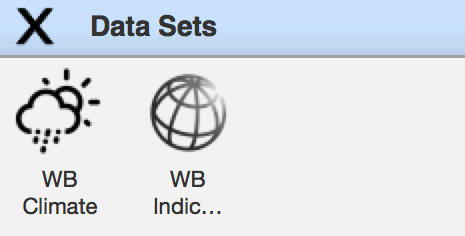
\includegraphics[width=4cm]{pic/data_sets_group.png}
  \end{center}
  \caption{Skupina gradnikov data sets}
  \label{drevo}
\end{figure} 


\subsection{wb indicators gradnik}

za sestavo smo si pomagali z gradniki Orange.gui 

elementi gradnika

2 osnovna filtra: 

- izbor indikatorjev ki se pokazejo v seznamu all/common/featured 
  ki ustreza seznamu indikatorjev na strani: 
  all - vse (tudi nekateri ki jih na strani ni nastetih)
  common - http://data.worldbank.org/indicator?tab=all
  featured - http://data.worldbank.org/indicator?tab=featured
- text filter

gradnik ima sistem za prikaz (progress bar?) 

moznost izbire tipa izhoda (countries in time series - opis)

\begin{figure}
\begin{center}
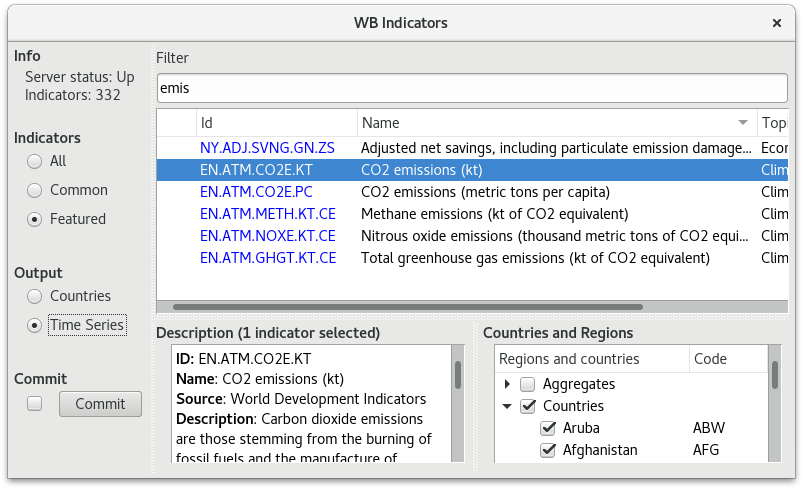
\includegraphics[width=12cm]{pic/co2_temp_indicator_selection.png}
\end{center}
\caption{Odločitveno drevo za izbor primerne metode.}
\label{co2_temp_indicator}
\end{figure} 



\subsection{wb climate gradnik}

dovoli izbiro posameznih drzav 

moznost izbire tipa izhoda (countries in time series - opis)
za razliko od indikator apija tukaj nismo dodali metapodatkov drzav 



\begin{figure}
\begin{center}
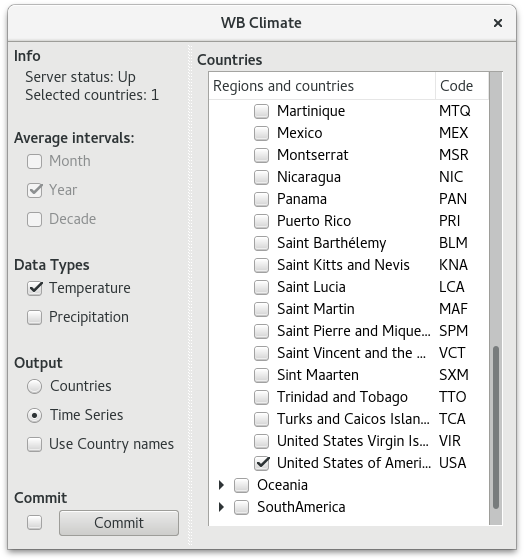
\includegraphics[width=12cm]{pic/co2_temp_climate_selection.png}
\end{center}
\caption{Odločitveno drevo za izbor primerne metode.}
\label{co2_temp_indicator}
\end{figure} 
